\documentclass[tikz]{standalone}
\usepackage{tikz}
\usetikzlibrary{bayesnet}
\begin{document}

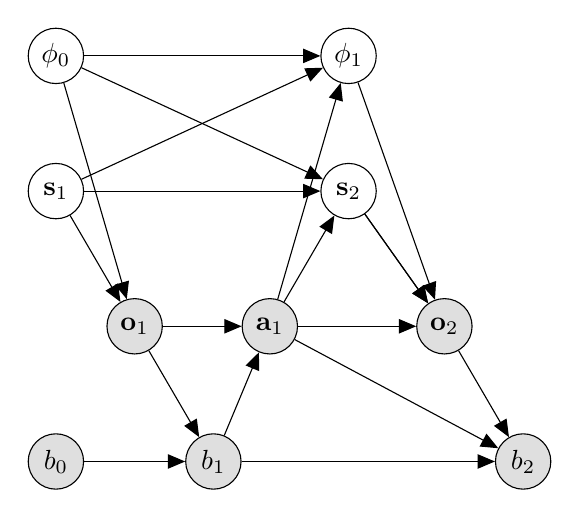
\begin{tikzpicture}

  % Define nodes
  \node[obs]                               (o1) {$\mathbf{o}_1$};
  \node[latent, above=of o1, xshift=-1cm]  (s1) {$\mathbf{s}_1$};
  \node[latent, above=of s1]               (phi0) {$\phi_0$};
  \node[latent, right=3cm of phi0]         (phi1) {$\phi_1$};
  \node[obs,    right=1cm of o1]           (a1) {$\mathbf{a}_1$};
  \node[obs,    below=of o1, xshift=-1cm]  (b0) {$b_0$};
  \node[obs,    below=of o1, xshift=1cm]   (b1) {$b_1$};
  \node[latent, right=3cm of s1]           (s2) {$\mathbf{s}_2$};
  \node[obs,    right=1.5cm of a1]         (o2) {$\mathbf{o}_2$};
  \node[obs,    below=of o2, xshift=1cm]   (b2) {$b_2$};

  % Connect the nodes
  \edge {s1,phi0} {o1} ;
  \edge {s2} {o2} ;
  \edge {o1,b1} {a1} ;
  \edge {phi0,s1,a1} {s2} ;
  \edge {phi1,s2,a1} {o2} ;
  \edge {b0,o1} {b1} ;
  \edge {b1,a1,o2} {b2} ;
  \edge {phi0,s1,a1} {phi1} ;

  % % Plates
  % \plate {yx} {(x)(y)} {$N$} ;
  % \plate {} {(w)(y)(yx.north west)(yx.south west)} {$M$} ;

\end{tikzpicture}

\end{document}